% id: 1292
% book: 라이트쎈 공통수학1 · 10 조합
% section: 실전 Training
% figure: tikz:fig-1292
% answer: $150$
% answer_source: 해설
% variant_level: 0 (원본 전사)
% 이 파일은 build.mjs 가 items.json 에서 만든다. 고칠 때는 items.json 을 고친다.
\hspace*{2mm}\begin{minipage}[t]{\dimexpr\linewidth-2mm\relax}\vspace{0pt}\smash{\raisebox{1.5mm}{\dmkichul{라이트쎈 공통수학1 1292번 · 180쪽}}}
\noindent\begin{minipage}[t]{0.58\linewidth}\vspace{0pt}\raggedright 오른쪽 그림과 같이 평행한 두 직선 $l$, $m$ 위에 각각 $6$개, $5$개의 점이 있다. 직선 $l$ 위의 점과 직선 $m$ 위의 점을 양 끝 점으로 하는 서로 다른 $2$개의 선분을 그을 때, 두 선분이 만나는 경우의 수를 구하시오. \cond{두 선분의 교점은 직선 $l$, $m$ 사이에 존재한다.}\end{minipage}\hfill\begin{minipage}[t]{0.4\linewidth}\vspace{0pt}\centering \resizebox{\ifdim\width>\linewidth\linewidth\else\width\fi}{!}{% 1292(본책 180쪽) — 평행한 두 세로 직선 l(왼쪽 · 점 6개), m(오른쪽 · 점 5개). 스캔 그림을 TikZ 로 다시 그림. 라벨은 원문의 l, m 만.
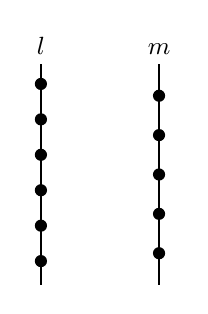
\begin{tikzpicture}[line width=0.6pt]
  \draw (0,-0.2) -- (0,2.6) node[above, font=\small] {$l$};
  \draw (1.5,-0.2) -- (1.5,2.6) node[above, font=\small] {$m$};
  \foreach \y in {0.1,0.55,1.0,1.45,1.9,2.35} { \fill (0,\y) circle (2.2pt); }
  \foreach \y in {0.2,0.7,1.2,1.7,2.2} { \fill (1.5,\y) circle (2.2pt); }
\end{tikzpicture}
}\end{minipage}\par\end{minipage}
